\documentclass{article}
\usepackage[T1]{fontenc}
\usepackage{lmodern}
\usepackage{graphicx}
\usepackage{amsmath,amssymb}
\usepackage[a4paper,margin=2cm]{geometry}
\usepackage[absolute,overlay]{textpos}
\setlength{\TPHorizModule}{1mm}
\setlength{\TPVertModule}{1mm}
\usepackage[indonesian]{babel}
\usepackage{hyperref}
\setlength{\emergencystretch}{2em}
% unit: Halaman 21

\begin{document}

% === Halaman 21 (llm) ===

\vspace{273.24mm}

\begin{verbatim}
void dekripsi()
{
    string plainteks, cipherteks;
    int i, k;
    char c;

    cout << "Ketikkan cipherteks: ";
    cin.ignore();getline (cin, cipherteks);
    cout << "Masukkan jumlah pergesaran (0-25): ";
    cin >> k;
    plainteks = ""; // inisialisasi plainteks dengan null string

    for (i=0; i < cipherteks.length(); i++) {
        c = cipherteks[i];
        if (isalpha(c)) {
            //hanya memproses alfabet
            c = toupper(c); // ubah karakter ke huruf besar
            c = c - 65; // kodekan huruf ke angka 0 s/d 25
            if (c - k < 0)
                c = 26 + (c - k); // kasus pembagian bilangan negatif
            else
                c = (c - k) % 26;
            c = c + 65; // kodekan kembali ke huruf semula
            c = tolower(c); // plainteks dinyatakan sebagai huruf kecil
        }
        plainteks = plainteks + c; // sambungkan ke plainteks
    }
    cout << "Plainteks: " << plainteks << endl; // cetak plainteks
}
\end{verbatim}

% deskripsi: Screenshot potongan kode program C++ untuk fungsi dekripsi cipher pergeseran.
% bbox normalisasi: [0.0400, 0.0400, 0.9500, 0.9600]
\begin{textblock*}{191.10mm}(8.40mm,11.88mm)
\noindent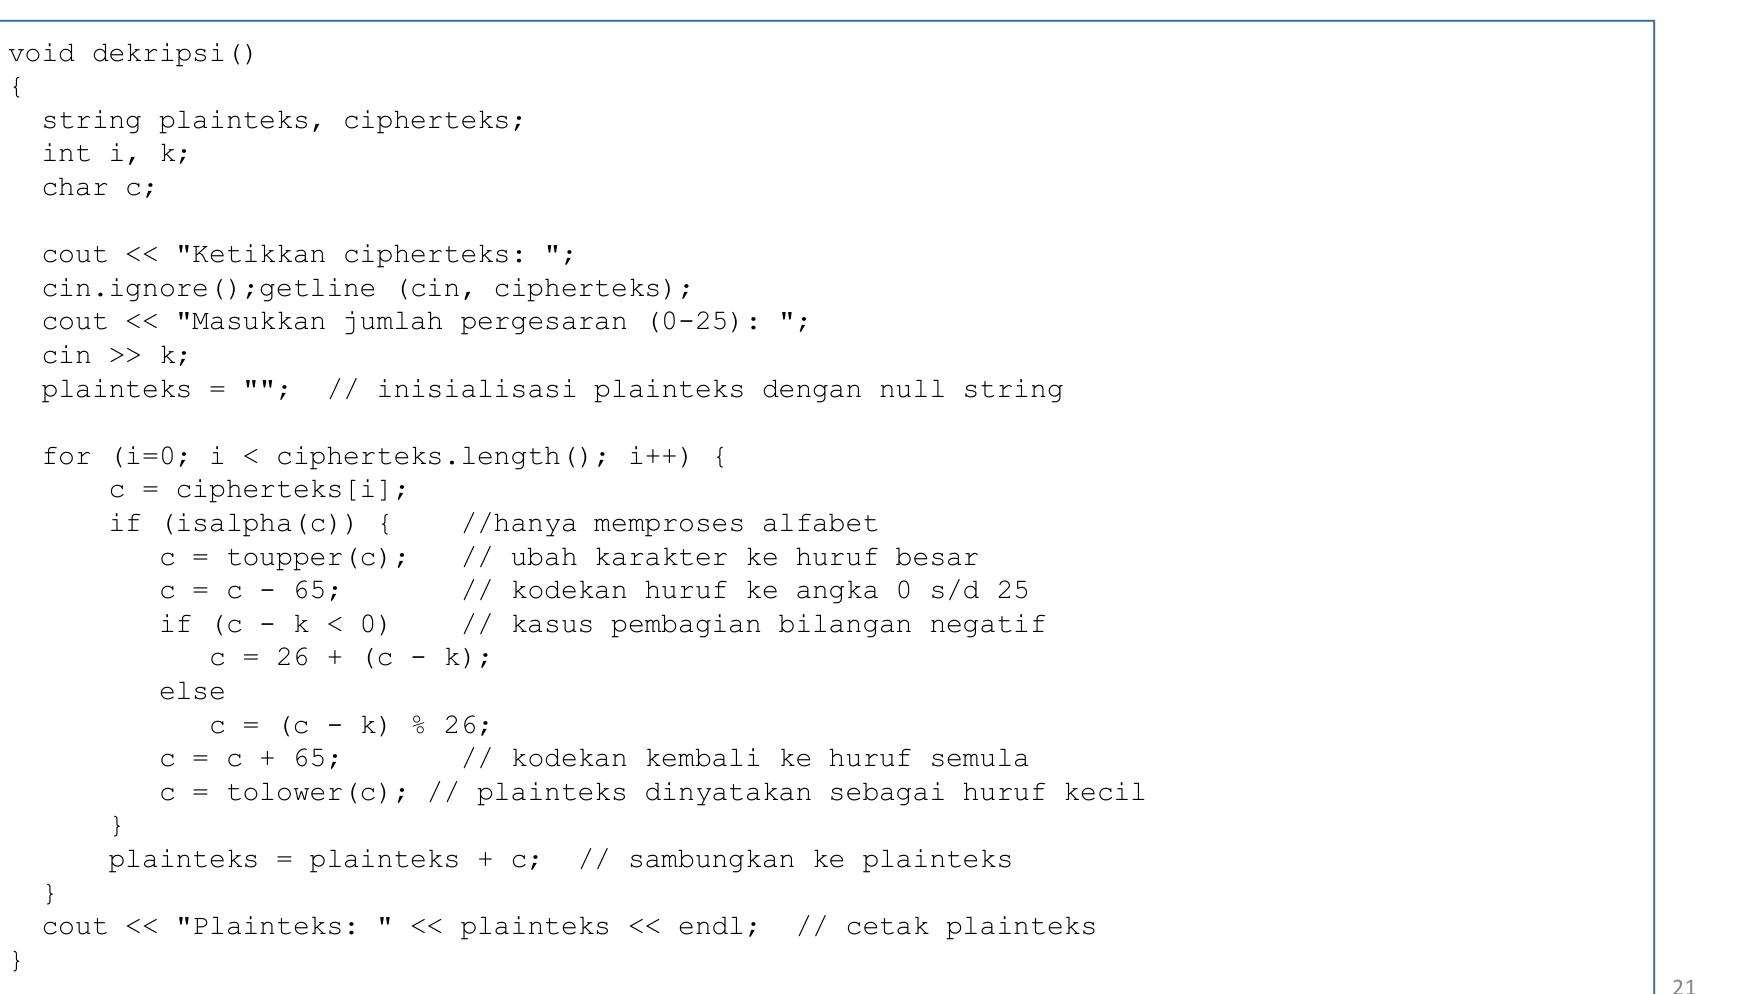
\includegraphics[width=191.10mm,height=273.24mm]{../../images/llm/page_021_img_01.png}%
\end{textblock*}

\end{document}
